% chapter 3: Dose Painting
\section{PET Imaging}
Dose painting tackles the inability of conventional radiation therapy to incorporate hypoxia into treatment planning by increasing the dose delivery to selected regions as indicated by images of tumour functional status. Positron emission tomography (PET) is a viable candidate for non-invasive hypoxia evaluation in tumour sites. The generation of PET images is based on the $\beta^+$ decay of a radiopharmaceutical, which is accumulated in hypoxic regions in the body. 
\subsection{$\beta^\pm$ decay}
In contrast to the energy spectrum of the $\alpha$ and $\gamma$ decay, the energy distribution of the $\beta$ decay is continuous. A continuous energy distribution is not compatible with a two body decay mechanism, which led to the postulation of a third particle by Pauli 1931 \cite{?}. The missing particle, the neutrino, was found by Cowan and Reines in 1956 \cite{?} explaining the continuous distribution of the $\beta$ decay as it now was interpreted as a three body mechanism. The $\beta$ decay can occure in three different versions.
\begin{enumerate}
\item $\beta^+$ \textit{decay: }For PET imaging, the $\beta^+$ decay is the most important one. It occurs when a proton decays into a neutron. As the proton is stable ($\tau_p > 2.1 \times 10^{29}$ years \cite{PDG}), the $\beta^+$ decay is only possible if the parent nucleus is in an excited state. If the binding energy of the parent nucleus is less than that of the daughter nucleus, this decay will not occur. In general, the $\beta^+$ decay scheme is as follows:
\begin{equation}
^A_ZX\rightarrow ^A_{Z-1}Y + e^+ \nu_e + Q.
\end{equation}
$\nu_e$ is the electron-neutrino and $Q$ is kinetic energy that is shared with all three particles. $X$ describes the parent nucleus and $Y$ the daughter nucleus.
\item $\beta^-$ \textit{decay: }The $\beta^-$ decay occurs if a neutron decays into a proton. In contrast to the $\beta^+$ decay, this decay is more common as the mass of the neutron is slightly higher due to its quark constituents. Therefore the mean lifetime of a neutron is much lower with $\tau = 881.5$s\cite{PDG}. The $\beta^-$ decay schema proceeds as follows:
\begin{equation}
^A_ZX\rightarrow ^A_{Z+1}Y + e^- \overline{\nu_e} + Q.
\end{equation}
\item \textit{Electron capture: }If the parent nucleus is not able to provide the energy necessary for a $\beta^\pm$ decay, it is possible that the nucleus will capture on of its orbital electrons. The electron itself usually originates from the K-shell to initialize the conversion of a proton into a neutron.
\begin{equation}
^A_ZX + e^-\rightarrow ^A_{Z-1}Y + \nu_e + Q.
\end{equation}
\end{enumerate}
\subsection{Physical principle of PET}
\begin{figure}[htp]
\centering
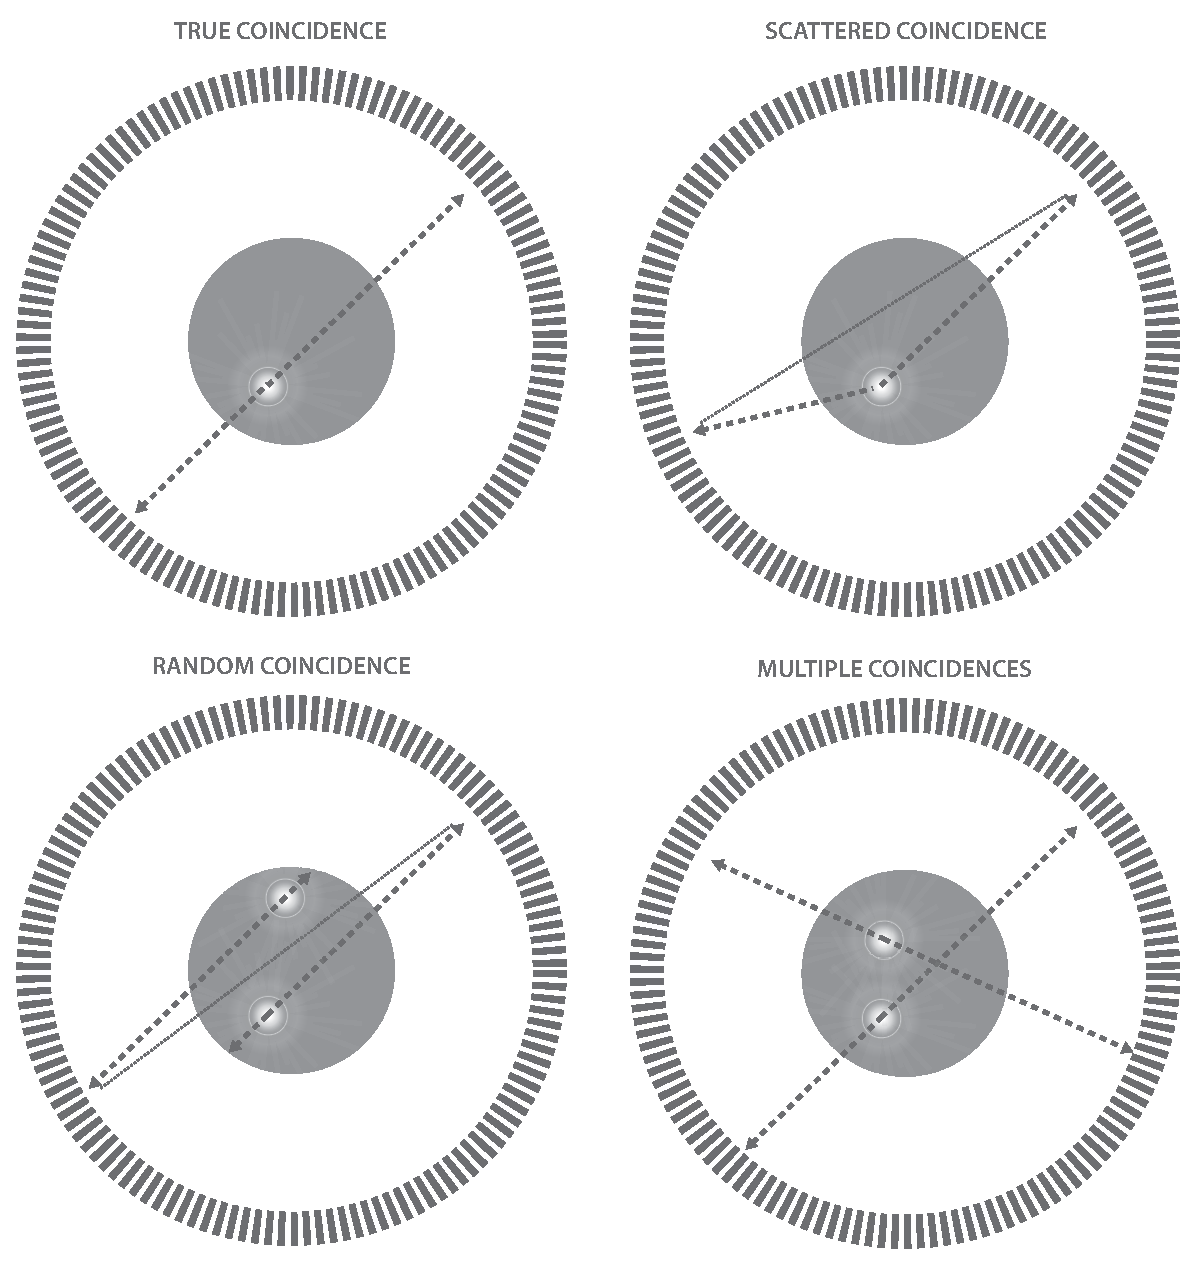
\includegraphics[scale = 0.7]{/Users/alex/Master/contents/images/Coincidence.eps}
\vspace{1cm}
\caption{Total cross section $\mu$ in units of barn (10$^{-28}$m$^2$) in the region from 1 eV up to 10 GeV. For radiotherapy, the Compton effect is most prevalent, as the common energies are in the range of a few MeV.}
\label{fig:coincidence}
\end{figure}
PET can be accomplished by administering a radionuclide tracer. In a biological environment, these radionuclide tracers undergo a $\beta^+$ decay. The positron gradually loses energy until it combines with an electron. The formation of an electron with a positron is called \textit{Positronium}. In general, the process of positron annihilation is more complex as it can happen in a variety of ways. About 2\% of positrons can annihilate before reaching thermal equilibrium to form positronium \cite{Heitler}. If a positron reaches thermal equilibrium, the strong Coulomb field of the nucleus averts it from annihilating with inner shell electrons of the atoms. Therefore, formation of positronium can only happen in three different situations: combination with free electrons, weakly bound electrons of the atoms outer shell or within low electric potentials between atoms of the molecule.\\Positronium can be created in two different versions, which is dependent on the spin configuration. The $^1$S singlet state is called \textit{parapositronium}, while the $^3$S triplet state is called \textit{orthopositronium}. Parapositronium has a half-life value of $\tau  \approx 125 \times 10^{-12}$s \cite{PDG}, creating a photon pair after its decay. In the centre of mass system of the Positronium at rest both photons are emitted back-to-back (emission angle of 180$^\circ$). The decay of parapositronium into two photons is more frequent due to its angular momentum. Orthopositronium has a spin of one and usually decays into three photons which is also more stable than it singlet brother with $\tau  \approx 140 \times 10^{-9}$s \cite{PDG}. The dominant process for the creation of photon pairs for the reconstruction of PET images, is parapositronium annihilation, as its cross section is 372 times larger \cite{Musiol}.\\By measuring both photons from the positronium decay with a ring of detectors, it is possible to reconstruct a \textit{line of response} (LOR). LORs are registered via coincidence detection. This means, if the PET scanner detects two photons within a set time window, a LOR is defined. The larger the density of LOR, the higher the accuracy in the reconstruction process of the PET image. Due to other physical processes and randomness of events, coincident detection can be divided into four categories, which can also be seen in figure \ref{fig:coincidence}:
\begin{enumerate}
\item \textit{True coincidence: }If the LORs cross the interaction point of the annihilation.
\item \textit{Scattered coincidence: }Photons may be scattered within the patient through the Compton effect. This leads to a shift in the LOR reconstruction. Due to their energy loss, it could be possible to reject these events since PET scanners operate in the energy regime of 350 keV up to 650 keV. The interaction of the photon via Compton scattering lowers the energy of the photon. Therefore, photons with larger scattering angles can be rejected to avoid scattered coincidences.\
\item \textit{Random coincidence: }Two annihilation events occur within a short time period, but only one photon from each interaction is registered in the PET scanner. Therefore one LOR is generated originating from two different annihilation events leading to random coincidence. 
\item \textit{Multiple coincidences: }If three or more photons are detected in the same time window in the PET scanner, multiple LORs can be reconstructed.
\end{enumerate}
In addition to the uncertainties in coinciding photon pairs, there is another problem that stems from an idealization of the positronium formation process. In theory, positronium is at rest when it reaches thermal equilibrium. However, normally positronium is not at rest in the centre-of-mass system. The additional energy from the binding process with its electron partner as well as the moving centre of mass reference frame can lead to a difference in energy of the two gamma rays of about 10 eV leading to \textit{non-collinearity}. Non-collinearity leads to a decay of positronium, where photons are not exactly back-to-back, which can lead to a mispositioned LOR. The usual deviation from the 180$^\circ$ back-to-back photon emission is about $\pm$ 0.25$^\circ$\cite{Cherry}.

\section{Quantification of hypoxia}
\subsection{Radiopharmaceutical approach to hypoxia assessment}\label{chap:tracers}
\begin{figure}[p]
\centering
\subfigure[FMISO]{

\includegraphics[scale = 1]{/Users/alex/Master/contents/images/FMISO.eps}
}
\hspace{0.3cm}
\subfigure[FDG]{

\includegraphics[scale = 1]{/Users/alex/Master/contents/images/FDG.eps}
}
\hspace{0.3cm}
\subfigure[Cu-ATSM]{

\includegraphics[scale = 1]{/Users/alex/Master/contents/images/CuATSM.eps}
}
\subfigure[FAZA]{

\includegraphics[scale = 1]{/Users/alex/Master/contents/images/FAZA.eps}
}
\hspace{0.3cm}
\subfigure[FETA]{
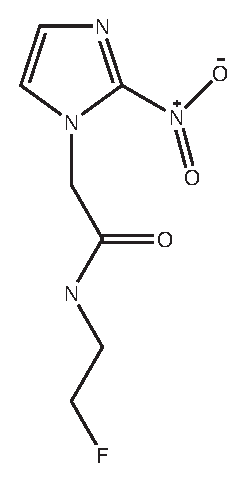
\includegraphics[scale = 1]{/Users/alex/Master/contents/images/FETA.eps}
}
\hspace{0.3cm}
\subfigure[FETNIM]{
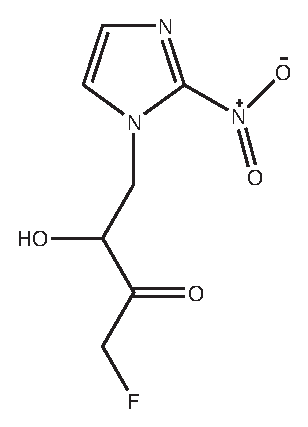
\includegraphics[scale = 1]{/Users/alex/Master/contents/images/FETNIM.eps}
}
\caption{Chemical structure of common tracers used in PET. FMISO and Cu-ATSM are commonly used in current studies, while studies with FAZA, FETA and FETNIM are on the way. FDG can be administered as a hypoxia tracer but is usually deployed for the use staging.}
\label{fig:hypoxiatracer}
\end{figure}
One of the major insights to hypoxia measurements via radiopharmaceutical tracers was achieved by the decryption of the N-alkyl-2-nitroimidazoles mechanism. This substance has been shown to be trapped in living cells that were hypoxic. Due to its electron affinity, the functional group of the 2-nitroimidazoles (-NO$_2$) can combine with an electron $e^-$ to form a radical anion (-NO$_2^-$). In presence of O$_2$ within the cell, the oxygen will be able to accept the electron from the nitro anion radical as oxygen has a higher electron affinity. If this happens, the nitroimidazole can return to its original form. If the nitro anion radical is able to react with another electron, the present O$_2$ is not able to reduce the nitroimidazole radical to its original form. The lack of oxygen will reduce it to a highly effective alkylating agent (RNH$_2$), as it will accept another electron. This mechanism leads to a higher cellular retention of the tracer.\\Tracer uptake is measured in standardized uptake values (SUV). The SUV can either be computed on voxel-wise basis or over a region of interest. SUV needs three different parameters to be calculated:
\begin{equation}
\mathrm{SUV}_i = \frac{c_i(t)}{c_0\cdot m}.
\end{equation}
Here $c_i(t)$ is the tissue radioactivity concentration in MBq/kg while $c_0$ is the radioactivity concentration at the time of the tracer injection. $m$ is the body weight of the patient. One of the reasons why SUV is not always a good means of measuring tracer uptake concentrations is related to $m$. While most authors use the body mass to normalize the SUV, others may use the lean body mass \cite{pmid8234714} or the body surface area \cite{pmid8271040}. Figure \ref{fig:hypoxiatracer} shows all discussed hypoxia tracers used for PET imaging.
\subsubsection{FMISO}
\begin{figure}[hb]
\centering
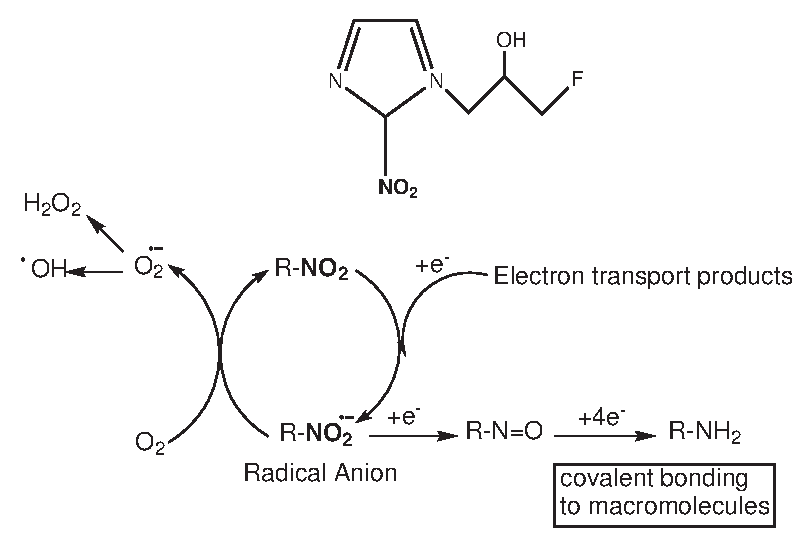
\includegraphics[scale = 1]{/Users/alex/Master/contents/images/MISORetention.eps}
\vspace{1cm}
\caption{Retention mechanism of FMISO in the environment of oxygen. Figure adopted from \textit{Krohn et a.}\cite{pmid18523070}.}
\label{fig:MISORetention}
\end{figure}
In PET one of the most common hypoxia tracers is [$^{18}$F]fluoromisonidazole (1-(2-nitroimidazolyl)-2-hydroxy-3-fluoropropane) or FMISO for short. Similar to misonidazole (MISO), FMISO will metabolize in the same way. Figure \ref{fig:MISORetention} shows the retention mechanism for FMISO. FMISO will use enzymes (xanthine oxidase, lipoxygenases and NADPH oxidases \cite{pmid18523070}) to create the single-electron product. While MISO is mainly metabolized in the liver, FMISO is not, due to its missing methoxy substituent.\\The imaging protocol for FMISO is arranged in such a way that the imaging process will begin 90-120 minutes after the injection of the radiopharmaceutical (quantity depends on patients weight). During the imaging process of about 20 minutes, a venous blood sample is drawn to normalize the static PET image data to the $^{18}$F concentration in blood. This is known as the tissue-to-blood ratio $T/B$. Normoxic tissues usually exhibit $T/B = 1$. Hypoxic tumour volumes are characterized by the maximum $T/B$, corresponding to the major hypoxic level. The hypoxic volume HV can be derived by adding up all voxels whose $T/B$ is larger than a set threshold \cite{pmid18523070}.\\The general discussion around hypoxia imaging is related to its accuracy of predicting correct pO2 values in tumour sites. Multiple studies have been conducted to prove or disprove a direct link between FMISO uptake and pO2 via invasive Eppendorf electrode pO2 measurements (cf. \ref{chap:eppendorf}). Due to the number of positive correlations shown in multiple studies, this work will assume this correlation to be true. This will allow a direct interpretation of FMISO SUV uptake value as hypoxia in PET imaging.
\subsubsection{FDG}
In contrast to FMISO, 2-deoxy-2-$^{18}$F-fluoro-D-glucose (FDG) is a non-imidazole imaging agent. FDG is generally used for staging. FDG uptake is dependent on the expression of proteins that are under control of HRF-1, which can, in some cases, be in good agreement with the hypoxia level. Multiple studies with direct pO2 measurements have shown that, in contrast to FMISO, FDG is unreliable when predicting hypoxia \cite{pmid18682937}. This is mainly because FDG is very sensitive to the metabolic state in cells. On the other hand the accumulation of FDG could also be used to derive the current metabolic state showing differences between normoxic and hypoxic cancer cells \cite{pmid17400370}. Multiple studies with the goal of showing a direct correlation between FDG uptake and hypoxia are inconclusive.
\subsubsection{Cu-ATSM}
$^{64}$Cu(II)-diacetyl-bis(N$^4$-methylthiosemicarbazone) (Cu-ATSM) is a hypoxia imaging agent that uses a metal complex of radioactive copper. Cu-ATSM can be reduced in a hypoxic environment to [Cu(I)-ATSM]$^-$. Due to its negative charge, it can be trapped within the cell. Multiple studies have been performed to show the hypoxia selectivity of Cu-ATSM retention toward cell hypoxia \cite{pmid9662602}. However a recent study with multiple cancer cell types has indicated that Cu-ATSM may not be a suitable hypoxia tracer for all tumour types \cite{pmid16741309}. The administration of Cu-ATSM plays a very important role in its ability to yield correct correlations between tracer retention and tumour hypoxia. Several studies showed that the tracer uptake of Cu-ATSM 4 hours after the injection will not correlate to FMISO uptake values, while a Cu-ATSM image after 16-20 hours will show a good correlation. Cu-ATSM and FMISO seem to yield common results, whereas FDG uptake is not correlated to Cu-ATSM in any way \cite{pmid12831991}.
\subsubsection{Other nitroimidazole hypoxia tracers}
\paragraph{FAZA: }In contrast to FMISO, 1-(5-deoxy-5-fluoro-(-D-arabinofuranosyl)-2-nitroimidazole (FAZA) is more hydrophilic. In general FAZA exhibits larger $T/B$ as well as tumour-to-muscle ratios $T/M$. This implies a higher signal for hypoxic regions in tumours and better differentiation between a background signal \cite{pmid12745023}. In measurements with Eppendorf polarographic needles, FAZA has proven to be consistent with tumour hypoxia \cite{pmid18313528}.
\paragraph{FETA: }$^{18}$F-fluoroetanidazole (FETA) was developed to circumvent metabolic side reactions from FMISO but was found to be a sophisticated hypoxia tracer. FETA has major advantages on the field of non-hypoxic degradation in vivo, as it appeared to be less metabolized \cite{pmid15150578}.
\paragraph{FETNIM: }$^{18}$F-fluoroerythronitroimidazole has been reported to show higher $T/B$ ratios for hypoxic tumour regions than FMISO \cite{pmid7862981}. In a clinical study on the abilities of FETNIM for hypoxia imaging, similar correlations between tracer uptake and hypoxia have been shown \cite{pmid14722675}. Until now FETNIM studies have been performed with head and neck cancer patients only.
\paragraph{EF: }The field of hypoxia tracer development is a large and constantly evolving field. Currently, multiple hypoxia tracers are developed as 2-nitroimidazole agents such as EF1 \cite{pmid10688119}, EF3 \cite{pmid17334763} and EF5 \cite{pmid12552344}. A study by \textit{Komar et al.} \cite{pmid18997048} showed that EF5 initial uptake is governed by blood flow, while the later phase uptake and binding is hypoxia-specific. Therefore EF tumour markers could hold new possibilities once approved.
\subsection{Modelling hypoxia with FMISO}
\begin{figure}[htb]
\centering
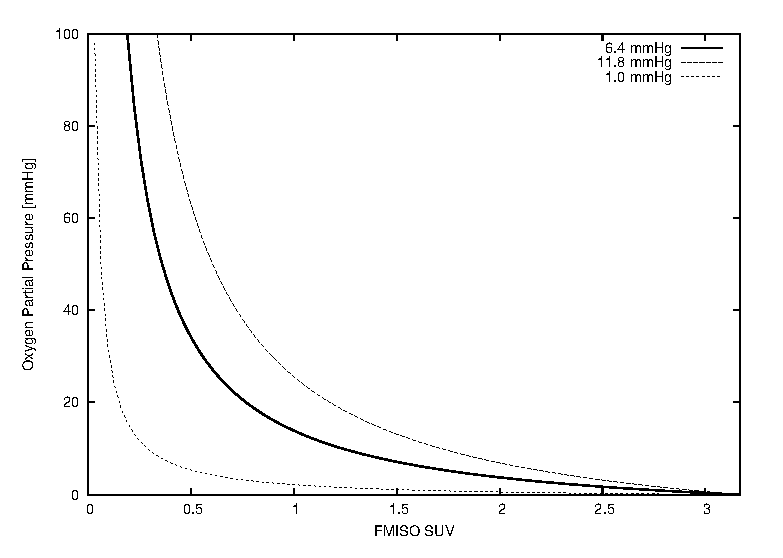
\includegraphics[scale = 1]{/Users/alex/Master/contents/images/pO2Model.eps}
\vspace{1cm}
\caption{Transformation of FMISO PET SUV to oxygen partial pressure derived from the parameters of the model developed by \textit{Chang et al.}\cite{pmid19994538} . Dotted and dashed line show the impact of the error of the model parameter $p_{50} = 6.4 \pm 5.4$ mmHg with due regard to the steepness of the transformation function. }
\label{fig:pO2Model}
\end{figure}
Hypoxia can be measured with the help of PET using a FMISO imaging agent as it has been found to be positively correlated with retention of nitroimidazol in hypoxic tumour cells. The degree of correlation between FMISO concentration (intensity) measured with EPT imaging and hypoxia is variable, but was generally found to be positively correlated. Therefore, in this work high FMISO retentions will be interpreted as highly hypoxic regions, whereas low FMISO retentions are considered more oxic. In a study performed by \textit{Chang et al} \cite{pmid19994538} FMISO PET uptake values have been directly compared to Eppendorf polarographic needle measurements to derive a model, which is able to relate these two quantities. The oxygen partial pressure (pO2) of the voxel $i$ can be derived by virtue of the FMISO retention $I_i$
\begin{equation}\label{eq:changmodel}
p_i = p_\mathrm{50}\left(\frac{I_\mathrm{max}}{I_i}-1\right).
\end{equation}
$I_\mathrm{max}$ is the maximum intensity (tracer concentration) in a PET image in a fully hypoxic environment (p=0 mmHg), while $p_\mathrm{50}$ is the oxygen partial pressure when the FMISO retention is the half maximum value. In the study by \textit{Chang et al.} \cite{pmid19994538} $p_\mathrm{50}$ could only be measured with low precision due to the high fluctuations in Eppendorf polarographic needle measurements
\begin{equation}
p_\mathrm{50} = 6.4 \pm 5.4 \mathrm{mmHg}.
\end{equation}
$I_\mathrm{max}$ on the other hand is dependent on the tracer and should be determined from to other clinical data, as this parameter could also be dependent on the tumour type and other factors.\\\textit{Bowen et al.} \cite{pmid21843774} proposed another approach to link tracer retentions directly to oxygen partial pressure values through electrochemical modelling. One of the major motivations to this approach was that tracer uptake and retention mechanisms in PET in vivo are difficult to compare. An electrochemical formalism was derived by describing the bioreductive retention mechanism of FMISO and Cu-ATSM under steady-state conditions to relate time-averaged activity concentrations to pO2 values. The approach works in two steps: First, tracer concentration is related to oxygen concentrations, which is transformed to pO2 values
\begin{equation}
\mathrm{pO2} = K_\mathrm{H}(T)\cdot 760 \frac{\mathrm{mmHg}}{\mathrm{atm}}[\mathrm{O}_2].
\end{equation}
The constant $K_H$ is the Henry coefficient which itself is dependent on the solution and temperature.  For FMISO and Cu-ATSM the different retention mechanism ultimately lead to different chemical transformation functions to calculate pO2 values from tracer uptake values. As the math and chemistry behind this electrochemical modelling is quite complex, the author will only present the final equation for FMISO
\begin{equation}
\mathrm{pO2}_\mathrm{FMISO} \approx \frac{K_\mathrm{H}}{K_\mathrm{NR}^3K_{\mathrm{O}_2}}\frac{760}{[\mathrm{FRNO}_2^{\bullet -}(O)]}[\mathrm{H}_2\mathrm{O}].
\end{equation}
Here $\mathrm{FRNO}_2^{\bullet -}(O)$ represents the concentration of the FMISO that is trapped by hypoxia in the tumour. $K_\mathrm{NR}$, $K_{\mathrm{O}_2}$ are constants derived from chemical consideration. \textit{Bowen et al.} also compared their electrochemical model to direct measurements with Eppendorf polarographic needles. In general this approach shows strong correlations with modelled distributions with lymph nodes, while primary tumour sites do not. Strong deviations in such volumes have been confirmed by another study by \textit{Piert et al.} \cite{pmid11150699}. In the latter, FMISO uptake has been investigated in vivo in porcine liver. The SUV was calculated from 659 single tissue samples and compared with the regional hepatic oxygen delivery calculated from the regional arterial and portal venous flow. Measurements of 121 liver tissue samples allowed a predictions of oxygen partial pressure from FMISO SUV
\begin{equation}
\mathrm{FMISO} = 1.05 + 6.7^{-0.117\cdot \mathrm{pO2}}\rightarrow \mathrm{pO2} = -4.49\cdot \log_{6.4}(\mathrm{FMISO - 1.05}).
\end{equation}
Although this model includes more clinical data than the model by \textit{Chang et al.} \cite{pmid19994538} it is less satisfactory as its functional form exhibits a singularity at 1.05. Furthermore, this model should not be applied to head and neck cancer patients, as the measured maximum SUV$= 2.28$ extrapolates an oxygen partial pressure of $p=-0.5$mmHg, which is unphysical. Therefore the model from \textit{Chang et al.}\cite{pmid19994538} will be deployed in this thesis.
\subsection{Correlation of tumour hypoxia vs. FMISO uptake values}\label{chap:hypoxiacorrelation}
In general a clear correlation between hypoxia and tracer retention in patients cannot be assumed. Multiple studies have been conducted in this area to find correlation between FMISO uptake and hypoxia. A direct measurement with invasive Eppendorf polarographic needles have confirmed a positive correlation between FMISO uptake and hypoxia \cite{pmid16104907, pmid16841141, pmid17598907, pmid15480509, pmid8892467}. In a detailed investigation by \textit{Gagel et al.} \cite{pmid17598907} multiple correlations of FMISO were cross referenced to direct Eppendorf measurements. While FDG did not exhibit any correlations to direct measurements, FMISO tumour to muscle ratios were found to be correlated. Although multiple studies point to the fact that hypoxia is correlated with FMISO uptake, it has also been shown that only human soft tissue exhibits such a correlation \cite{pmid12865184}. A study conducted by \textit{Mortensen et al.} \cite{pmid20831480} examined the association between measured hypoxia defined by a FMISO PET image and Eppendorf pO2 electrodes.  A total of of 18 patients was processed by creating virtual voxels as localization for pO2 electrodes as well as FMISO scans. In general, tumours could be categorized in three groups: Well oxygenated with good agreement between FMISO uptake and direct measurements, hypoxic tumours with the same outcome and hypoxic tumours that did not show any concordance between assays. In general more hypoxic tumours were measured to be more hypoxic with a direct measurement than with a FMISO PET scan. As head and neck tumours are generally more hypoxic, this could lead to an underestimation of the FMISO signal and to failure of local tumour control  despite dose painting. Due to the number of positive correlations found between FMISO uptake and hypoxia, this thesis will make the assumption that FMISO uptake is positively correlated with hypoxia.
\subsection[Eppendorf polarographic needle electrodes]{Measuring hypoxia with Eppendorf polarographic needle electrodes}\label{chap:eppendorf}
PET imaging using on of the various hypoxia tracers described in chapter \ref{chap:tracers} is a non-invasive way to assess tumour hypoxic. An invasive method for direct measurements of the oxygen level of tissue and tumour volumes are Eppendorf polarographic needle electrodes (cf. figure \ref{fig:eppendorf}). The technical structure of such an electrode can differ from the model, but it generally is manufactured as a stainless steel shaft with a lancet shaped tip. The tip contains a membranized polarographic recessed microcathode (gold wire) \cite{pmid8018370}.\\The measurements conducted with such an electrode represent an average oxygen partial pressure of the probed environment. The average value includes all cells in the intercellular environment that are in the sampling range of the probe. This might also include necrotic as well as living tissue. The usual procedure of measurements with Eppendorf electrodes includes the administration of an anaesthetic (lidocaine) with a subsequent insertion of an indwelling cannula. Afterwards removal of the trocar (medical instrument with a sharply pointed end used together with a hollow cylinder to be introduced into blood vessels, especially for laparoscopic surgeries), the needle electrode can be guided through the tissue. One measurement consists of predetermined distance which is then moved step by step (size variable) through the tumour volume, which is done automatically. The more tracks are acquired, the smaller the error on the measured value. 
\begin{figure}[hbt]
\centering
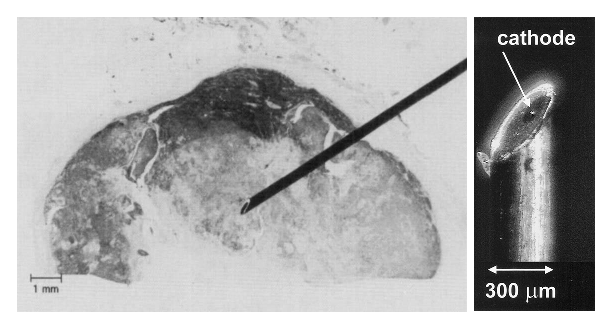
\includegraphics[scale = 1.2]{/Users/alex/Master/contents/images/eppendorf.eps}
\vspace{1cm}
\caption{(Left) Eppendorf polarographic needle electrode in a section of neck node metastasis taken from \textit{Nordsmark et al.}\cite{pmid8018370}. (Right) Close up of an Eppendorf electrode taken from \textit{Seddon et al.}\cite{pmid11352767}}
\label{fig:eppendorf}
\end{figure}
\section{Review of dose painting methods}
The deployment of PET has increased in the past years, mainly because PET has revolutionized imaging by giving radiation therapist a tool for anatomic localization of functional abnormalities in the complex territory of tumours. PET is used for staging, detection of unknown primaries and monitoring of treatment results. Dose painting is one the major concepts that involves the usage of PET to improve treatment planning. All dose painting approaches use a functional image such as PET or MRI to derive a dose escalation in one or the other way to account for hypoxic regions in tumour volumes. The way how the escalation is calculated can vary. Until now, dose painting by numbers (DPBN) has been used to prescribe a physical dose to hypoxic tumour volumes. The way how additional dose is prescribed to a clinical dose can be determined in various ways. This chapter will comment on all different dose painting methods used to overcome hypoxia.
\subsection{Binary dose escalation}
Binary dose escalation uses PET imaging to identify hypoxic tumours. If a lymph node or the primary tumour has a high tracer uptake value, it is considered to be hypoxic. The intensity of the imaging agent does not scale the additional boost that is administered in the this area. Therefore binary dose painting dose not incorporate any biological basis for the prescription. Multiple studies have been performed with this approach \cite{pmid20855118, pmid11240261, pmid17869020, pmid19203843}.\\One of the major findings derived from binary dose painting is that dose escalations can be achieved in most patients without compromising the dose limits to critical structures. Some cases were considered not the be feasible with this approach as they had critical organs (brainstem or spinal coord) very close to the target volumes \cite{pmid20855118}. In a study performed by \textit{Chao et al.} \cite{pmid11240261} using an Cu-ATSM imaging agent results showed feasibility of dose escalations in hypoxic sub volumes in head and neck cancer, without compromising OAR constraints. While the GTV was treated with a dose of 70 Gy, its hypoxic sub volume was treated with a dose of 80 Gy. Another study conducted by \textit{Lee et al.} \cite{pmid17869020} using FMISO guided IMRT found that dose escalations could easily be increased to 84 Gy (based upon a 70 Gy original prescription) and up to 105 Gy in one patient, without exceeding dose limits for critical structures. 
\subsection{Functional dose escalation}
Functional dose escalations use a prescription function to calculate dose escalations. The way how the functional image is interpreted and incorporated into the treatment planning process are quite different from their implementation.
\begin{itemize}
\item \textit{Cost function manipulations: }:  Rather than manipulating the dose prescription directly, this approach featured a dose efficiency $e(\vec x)\in[0,1]$, which was coupled with the dose-based cost function of the optimization algorithm to incorporate functional images such as PET. This way, the dose-based cost function $F(d(\vec x))$ was replaced with $F(d(\vec x)e(\vec x))$ instead. The analytical form of $e(\vec x)$ is very important since it will directly alter the way how the biological image will change the results of treatment planning. In a study performed by \textit{Alber et al.} \cite{pmid12587912} this function was rather simple as it represented a linear transformation of the signal intensity above a signal threshold
\begin{equation}\label{eq:alber}
e(\vec x) = 
\begin{cases}
\frac{1}{D_{\mathrm{Max}}}\left(D_{\mathrm{p}} +\frac{D_{\mathrm{max}}-D_{\mathrm{p}}}{I_{\mathrm{mean}}+I_{\mathrm{max}}}(i(\vec x)-I_{\mathrm{max}})\right) & I\geq I_{\mathrm{mean}}\\
1 & I< I_{\mathrm{mean}}.
\end{cases}
\end{equation}
Here $D_{\mathrm{Max}}$ is the maximum dose, $D_{\mathrm{p}}$ the prescribed dose, $I_{\mathrm{mean}}$ the mean intensity, $I_{\mathrm{max}}$  the maximum intensity of the functional image and $I(\vec x)$ the intensity at position $\vec x$. This simple prescription function is safeguarded against unreasonable dose escalations as it will use a linear prescription mechanism. On the downside, this functional prescription does not incorporate the underlying biology in a patient that can be acquired through PET.
\item \textit{Direct dose escalations: }Rather than manipulating the objective function in the treatment planning system to incorporate functional imaging it is possible to directly manipulate dose escalations. The magnitude of changes that are induced by such a dose escalation are dependent on the analytical form of the escalation function. Multiple studies have proposed different approaches to this problem. \textit{Bentzen et al.}\cite{pmid21356478} used a linear interpolation method
\begin{equation}\label{eq:bentzen}
D(I) = D_{\mathrm{Min}} + \frac{I-I_{\mathrm{Min}}}{I_{\mathrm{Max}}-I_{\mathrm{Min}}}\left(D_{\mathrm{Max}}-D_{\mathrm{Min}}\right).
\end{equation}
The dose escalation method proposed in equation \ref{eq:bentzen} has also been used in an adaptive dose painting study performed by \textit{Duprez et al.} \cite{pmid20643512} to create an FDG PET intensity based voxel-specific dose painting and has shown promising results in terms of feasibility. In a corresponding study, \textit{Madani et al.} \cite{pmid21742392} determined the maximum tolerated dose (MTD) in a phase I trial with 21 patients. The escalated median dose was elevated up to 80.9 Gy in the CTV and 85.9 Gy in the GTV. All surviving patients did not show any grade $\geq 4$ toxicity (life threatening or disabling side-effects) during treatment and follow-up, with the exception of mucosal ulcers. \\In general equation \ref{eq:bentzen} and equation \ref{eq:alber} use the same kind of linear transformation to incorporate functional imaging into the optimization process. Nevertheless, the level of impact can be quite different, as the latter directly manipulates the optimization process in the objective function, while \textit{Bentzen et al.} use dose scaling. \textit{Flynn et al.} \cite{pmid18635895} used a slightly different formula, which incorporated a linear scaling to dose boost $D_{\mathrm{Boost}}$ added on top of the original dose prescription $D_\mathrm{CTV}$ in the clinical target volume
\begin{equation}
D(I) = D_\mathrm{CTV} + \frac{I}{I_\mathrm{Mean}}D_\mathrm{Boost}.
\end{equation}
\end{itemize}
Physical dose painting that relies on a direct functional interpretation of the PET intensity, does not incorporate any considerations for the underlying biology. Therefore dose escalations are arbitrary as well as dependent on the functional form of the prescription function. \textit{Bowen et al.} \cite{pmid19218733} performed a study on the sensitivity of IMRT dose optimization to the mathematical form of a biological imaging-based prescription function. Polynomial functions were tested to simulate a continuous prescription, while sigmoidal functions were used to account for a threshold scenario. In addition two concepts were checked with both functions:
\begin{enumerate}
\item Prescribe a constant integral dose in the primary tumor volume.
\item Prescribe a maximum boosted dose to the primary tumour volume without fulfilling any integral dose constraints.
\end{enumerate}
\paragraph{Polynomial functions: }In general, polynomial functions represent a continuous prescription scenario. Depending on the exponent in the polynomial, the behaviour of prescription may change in different situations. A dose distribution planned using a square root function most closely resembles its prescription due to the smoothing of the dose gradients at higher dose boosts and the tighter distribution of prescribed dose about its mean. Square root functions therefore prescribe lower dose escalations to larger fractions of the PTV. On the other hand, a dose distribution resulting from the use of a quadratic prescription function least resembles its prescription due to the sharpening of these same dose gradients at higher dose boosts and larger spread in the distribution of prescribed dose about its mean. Quadratic prescription functions prescribe a higher dose to a smaller volume fraction. Therefore it becomes more and more difficult to deliver conformal dose distributions as the boost volumes become smaller in comparison to the treatment volume \cite{pmid17921573}.
\paragraph{Sigmoidal functions: }This function type is compatible with a threshold scenario. Sigmoidal functions are shaped with two parameters: slope and threshold position. Both parameters are not independent of each other, as changes in dose delivery are dependent on alterations in slope and the position of the threshold.  Increasing the prescription sigmoid slope at low threshold position yields to boosting of an increasing volumetric fraction of the PTV, while imposing steep gradients at the edges. Shifting the threshold towards a more central position, the dependence on the prescription slope becomes significant. Each voxel is equally sensitive to the steeper dose gradients, which causes smearing of the delivered dose as well as severe overdosed and underdosed regions \cite{pmid17921573}. 
\subsection{Dose painting by numbers via kinetic models}
Although most of the dose painting methods above can be categorized under the term 'dose painting by numbers', all of them lack the direct connection to a biological motivation for dose escalation. In a planning study by \textit{Thorwarth et al.} \cite{pmid17448882} hypoxia was incorporated into a new DPBN approach. Three plans were created to evaluate the outcome of DPBN: A conventional IMRT plan, a uniform dose escalation (binary dose painting) and hypoxia DPBN. The latter was nested into a planning framework by creating dose escalation factors (DEF) from a kinetic compartment model \cite{pmid15876662}. The model described the behaviour of FMISO trapped in hypoxic cells and its diffusion in interstitial space. This allows for a better identification of severely hypoxic and necrotic tissue than with SUV. DEFs were calculated with regard to local cell survival $M_i$ through a TCP model \cite{pmid16321146}
\begin{equation}
M_i = \exp\left(\frac{b\cdot \mathrm{TR}_i}{\mathrm{VP}_i+c}\right),
\end{equation}
where $\mathrm{TR}_i$ and $\mathrm{VP}_i$ are the tracer retention and vascularization-perfusion parameters for the $i$th voxel. The parameters $b$ and $c$ are acquired through the TCP model. Once the local cell survival $M_i$ is calculated, DEF can be calculated based on the mean radio sensitivity parameter of the linear quadratic model $\alpha$.
\begin{equation}
\mathrm{DEF}_i = \frac{\alpha D}{\alpha D - \ln M_i}.
\end{equation}
Here $D$ is the prescribed dose in the tumour volume. In the corresponding planning study, dose escalation was limited to 2.4 Gy per fraction, which was equal to DEF=1.2. DPBN via kinetic modelling assigns dose escalations of 2.2 Gy per fractions on small sub volumes that have a significantly higher survival due to hypoxia. DEF may vary on a larger scale from 1.03 up to 1.66, leading to problems with the limited dose of 2.4 Gy per fraction. This is mostly due to a combination of severe hypoxia and low vascularization and perfusion. This approach has been reevaluated in a later study by comparing predicted survival from the kinetic model with a FMISO PET image after 20 Gy direct evaluation \cite{pmid18524387}.
\subsection{MRI dose painting}
In contrast to the above discussed approaches to dose painting, \textit{Sovik et al.} \cite{pmid17674980} used dynamic contrast enhanced magnetic resonance (DCEMR) images to derive oxygen distribution. The distributions were created by inferring a direct proportionality of the time-averaged tracer concentration at a given point in the patient to the oxygen partial pressure in this region. The results were split into four compartments following the range of $p>20$ mmHg, $p=5-20$ mmHg, $p=[0.5-5]$ mmHg and $p = 0-0.5$ mmHg. Rather than escalating the dose in hypoxic regions of the tumour, dose redistribution around a mean dose $D_\mathrm{mean}$ was used
\begin{equation}
D_\mathrm{mean} - \sum\limits_{i=1}^NV_{ij}D_{ij} = 0,
\end{equation}
where $N$ is the number of compartments in the tumour, $V_{ij}$ the volume fraction of the compartment $i$ at treatment fraction $j$. This study applied IMRT to achieve the dose gradients needed from the guidance of the tumour map. It showed that IMRT dose distributions are less steep than the prescribed ones, as dose gradients are not completely  achievable with IMRT. This fact will become important for the approach that will be proposed in this thesis, as the same behaviour is shown. In the study, dose in compartments with high pO2 values was too high, while compartments with lower pO2 values was to lower. The compartments that were assigned to oxygen partial pressure between 5 mmHg and 20 mmHg, approximately matched the prescriptions. The major drawback on this dose painting approaches is the application of a compartment model used to categorize hypoxia levels with their corresponding assignment of dose redistribution. \textit{South et al.} \cite{pmid19928068} investigated the relationship between the complexity of the dose prescription and the tumour control probability. The results show, that most heterogeneous biological distributions divided by a few dose levels compartments show the beneficial tumour control. However, this is only true, when the prescribed dose level and the compartment geometry is well chosen. Therefore, the usage of compartments might show unpredictable behaviour in contrast to a method that does not rely on the quantization of dose level compartments.
\section{Novel approach: biological dose painting}
Hypoxia reduces radio sensitivity and if it is not properly accounted for, leads to overestimation of cell kill. With the help of the optimization of the biological effect and incorporation of HRF into the model, it is possible to overcome hypoxia and create an adaptive method to increase cell kill in those areas by dose escalations. The model applied in this approach has been described in detail in chapter \ref{chapter:2} and are combined in this chapter a novel approach of biological dose painting.
\subsection{Implementation of biological dose painting in KonRad}
The first step in biological dose painting is to convert the SUV uptake values to oxygen partial pressure via equation \ref{eq:changmodel}. This oxygen partial pressure can then be transformed to a HRF for every voxel with equation \ref{eq:hrfmodel}. Afterwards, a prescribed biological effect is calculated based on the prescribed physical dose. In a third step, the optimization begins to use the quadratic biological function to find the best possible treatment plan with due regard to normal tissue constraints as well as the biological effect prescriptions. Within every optimization step, the delivered effect $\varepsilon_D$  is evaluated for every voxel. $\varepsilon_D$ is calculated with
\begin{equation}
\varepsilon_D = \frac{\alpha_X}{\mathrm{HRF}}D+\frac{\beta_X}{\mathrm{HRF}^2}D^2,
\end{equation}
where $D$ is the current dose in the voxel. The optimization stops if the relative value change of the biological optimization function is less than 0.01 in the last 6 optimization steps. The resulting physical dose distribution is analyzed to make plan comparisons simpler\\As seen in equation \ref{eq:dosecompensation}, the optimizer will compensate for hypoxia by scaling the dose linearly with the HRF. In most cases normal tissue constraints will limit the possibility of dose escalation in hypoxic volumes (cf. chapter \ref{chapter:4}).
\subsection{Clinical tumour hypoxia}\label{chap:tumourhypoxia}
In a meta-study by \textit{Jens Overgaard} \cite{pmid21511351} a total of 4805 patients with head and neck cancer were reviewed in terms of dose boosting in radiotherapy. In general, overall hypoxic modifications of radiotherapy will result in therapeutic benefits as it increases local regional control. This was also found to be independent of the type of modification used to circumvent the high radioresistance of hypoxic tumour areas. In order to estimate a realistic treatment environment for dose painting the first step is to evaluate Eppendorf polarographic needle measurements in head and neck cancer patients. A total of 551 patients have been found through comprehensive literature search. In most studies, pO2 values were separately measured in primary tumour volumes and lymph nodes. Every study presented in table \ref{tab:po2parameter} (if not noted otherwise) has conducted an evaluation of regions with pO2 $\leq 2.5$mmHg and $\leq 5.0$mmHg, as well as a mean pO2 value. In general primary tumours and lymph nodes do not seem to deviate in mean value or volume distributions of hypoxia. Therefore there should be no differentiation in treatment approaches for these two targets. The mean value pO2 value in head and neck cancer has been measured as $10.36 \pm 2.04$ mmHg. The hypoxia levels have been measured as $16.09 \pm 4.65$\% with $\leq 2.5$mmHg and  $36.38 \pm 6.80$\% with $\leq 5.0$mmHg. This shows that head and neck tumours are generally hypoxic and hold a small fraction of highly hypoxic cells, which could lead to failure of local tumour control. Likewise, the range of mean values and volume percentages measured can be very large. Therefore it is important to customize the treatment for every patient which requires a deeper understanding in the link between FMISO tracer uptake values and the underlying oxygen partial pressure (cf. chapter \ref{chap:hypoxiacorrelation}). One of the goal of this thesis is to proof feasibility of dose painting in head and neck cancer patients. Therefore, all patients presented in this work, will be treated as an average hypoxia patient. The following assumptions are made for all patients:
\begin{itemize}
\item Every patient investigated in this thesis is assumed to exhibit the same hypoxic properties.
\item Only the gross tumour volume (GTV) is hypoxic. 
\item The GTV exhibits a mean oxygen partial pressure of 10mmHg. Sub volumes encompassed by the GTV hold voxels that are more hypoxic and represent the 5.0mmHg and 2.5mmHg levels (cf. chapter \ref{chap:tumourhypoxia} for detail construction of hypoxic volumes).
\end{itemize}
As patients are treated with radiation, the underlying biology changes. In terms of hypoxia, the biggest impact is associated with reoxygenation. The investigations of \textit{Lartigau et al.}\cite{pmid9797698} and \textit{Stadler et al.}\cite{pmid9783887} have shown that reoxygenation can clearly be measured after 32 Gy and 30 Gy respectively. In the study by \textit{Lartigau et al.} the mean oxygen partial pressure change up to 58\%, while the size of the highly hypoxic volume ($\leq 2.5$mmHg) shrunk from 14\% to 5\%. The same behaviour was observed in the measurements of \textit{Stadler et al.}. In primary tumour sites, the mean oxygen partial pressure increased up to 25\%, while the $\leq 2.5$mmHg and $\leq 5.0$mmHg volumes did not see any decrease. However, hypoxic volume reduction can be deduced by looking at the decreased statistical error on the volume measurements. 
\begin{sidewaystable}[p]
\centering
\small
\begin{tabular}{lccccc}
\toprule
\multicolumn{3}{c}{Study Information} & \multicolumn{3}{c}{pO2 Data [Range]}\\
\cmidrule(r){1-3} \cmidrule(r){4-6}
Study by & Type & Patients & Mean [mmHg] & $\leq$ 2.5 mmHg [\%] & $\leq$ 5.0 mmHg [\%]\\\\
\midrule\\
\textit{Becker et al.}\cite{pmid9765692}		& PT & 23 &  12.37 $\pm$ 10.18 [0.2-58.5] & 18.03 $\pm$ 22.54 [0.0-73.1] & 25.97 $\pm$ 38.64 [0.0-86.2]\\
									& LN & 22 &  13.71 $\pm$ 12.94 [1.9-50.3] & 18.56 $\pm$ 21.92 [0.0-66.0] & 27.86 $\pm$ 25.78 [0.0-88.5]\\
									& M & 30 &  43.78 $\pm$ 10.11 [20.8-67.7] & 0.36 $\pm$ 0.94 [0.0-5.1] & 0.95 $\pm$ 1.45 [0.0-7.6]\\\\
\textit{Lartigau et al.}\cite{pmid8453553}		& LN & 9 & 14.67 $\pm$ 11.86 [0.0-39.0] & 18.95 $\pm$ 30.04 [0.0-100.0] & -\\\\
\textit{Lartigau et al.}\cite{pmid9797698}		& C & 14 & 18.37 $\pm$ 12.81 [1.5-38.0] & 14.11 $\pm$ 18.02 [0.0-60.0]$^*$& -\\
									& C (32 Gy) & 14 & 28.92 $\pm$ 28.77 [3.0-100.0] &  4.89 $\pm$ 8.74 [0.0 - 30.0]$^*$& -\\\\
\textit{Nordsmark et al.}\cite{pmid16098619}	& C & 397 & 10.375 $\pm$ 3.57 [0.0-62.0] & 16.26 $\pm$ 9.01 [0.0-95.0] & 33.50 $\pm$ 14.24 [0.0-100.0]]\\\\
\textit{Stadler et al.}\cite{pmid9783887}		& PT & 2 & 7.50 $\pm$ 5.50 [2.0-13.0] & 25.50 $\pm$ 24.5 [1.0-50.0] & 38.50 $\pm$ 31.5 [7.0-70.0]\\
									& LN & 21 &  19.48 $\pm$ 15.33 [0.0-47.0] & 23.24 $\pm$ 20.47 [0.0-76.0] & 33.67 $\pm$ 26.68 [0.0-92.0]\\
									& PT (30 Gy) & 3 &  9.34 $\pm$ 3.40 [6.0-14.0] & 26.34 $\pm$ 12.12 [10.0-39.0] & 38.00 $\pm$ 9.89 [24.0-45.0]\\
									& LN (30 Gy) & 16 &  10.0 $\pm$ 11.13 [0.0-35.0] & 35.75 $\pm$ 23.38 [0.0-68.0] & 46.32 $\pm$ 22.90 [0.0-70.0]\\\\
\bottomrule\\
\textbf{Combined (PT)} & & 28 & 9.10 $\pm$ 2.79 [0.0-58.5] & 24.64 $\pm$ 9.79 [0.0-100.0] & 37.37 $\pm$ 9.17 [0.0-92.0]\\\\
\textbf{Combined (LN)} & & 68 & 12.77 $\pm$ 6.28 [0.0-50.3] & 24.38 $\pm$ 11.62 [0.0-76.0] & 37.37 $\pm$ 9.17 [0.0-100.0]\\\\
\bottomrule\\
\textbf{Combined (All)}$^\#$ & & 551 & 10.36 $\pm$ 2.04 [0.0-100.0] & 16.09 $\pm$ 4.65 [0.0-76.0] & 36.38 $\pm$ 6.80 [0.0-100.0]\\\\\\
\end{tabular}
\caption{pO2 values for different head and neck studies. All pO2 values were acquired with the help of Eppendorf polarographic needle measurements (if not stated otherwise). Errors are standard deviation of the given data and sample size. Combined data are gather through weight of standard deviation and number of patients screened. C = Combined (Tumor \& Nodes), LN = Lymphnodes, M = Muscle Tissue, PT = Primary Tumor. Remarks: $^*$ $\leq$ 2.0 mmHg, $^\#$ not including muscle tissue pO2 values}
\label{tab:po2parameter}
\end{sidewaystable}
\subsection{PET imaging}\label{chap:petimaging}
A comprehensive literature search has been conducted to evaluate the uptake values of FMISO and FDG tracers in head and neck cancer. In total 122 patients with FDG and FMISO images have been investigated. Most of studies presented in table \ref{tab:suvparameter} have been able to examine the uptake values of FMISO and FDG. Tracer uptake was characterized by using the maximum and mean tissue radioactivity concentration $c_i(t)$ to derive SUV. In general FDG uptake is higher than FMISO. Mean FDG SUV have been measured as $SUV_\mathrm{mean}=3.75 \pm 0.24$, while maximum SUV is  $SUV_\mathrm{max}=9.63 \pm 1.1$. For FMISO these values can be quantified with $SUV_\mathrm{mean}=1.76 \pm 0.16$ and $SUV_\mathrm{max}=2.28 \pm 0.32$. The found results for PET images with FDG and FMISO are used to make the following assumptions for further investigations in this thesis:
\begin{itemize}
\item PET images will are assumed to represent FMISO uptake distributions.
\item The maximum SUV=2.28 is assigned to the highly hypoxic regions in head and neck cancer. Therefore, if the FMISO SUV is equal to 2.28, a 2.5 mmHg oxygen partial pressure is inferred in this voxel.
\item To incorporate the maximum SUV correlation to 2.5 mmHg hypoxia levels, the pO2 model from equation \ref{eq:changmodel} has to be modified to account for this assumption. This can be easily done by changing the $I_\mathrm{max}$ to its  appropriate value, such that an intensity of $I=2.28$ yields $p=2.5$ mmHg
\begin{equation}
2.5\mathrm{mmHg} = 6.4\mathrm{mmHg}\left(\frac{I_\mathrm{max}}{2.28}-1\right) \rightarrow I_\mathrm{max} = 3.17 \pm 0.77.
\end{equation}
\end{itemize}
Just as with direct measurements of oxygen partial pressure, reoxygenation can be clearly seen in a study conducted by \textit{Eschmann et al.}\cite{pmid17543402}. It was found that the FMISO uptake after a total dose of 45 Gy decreased about 30\%, while the range of FMISO SUV change from 1.7-4.4 to 1.4-3.0. As lower FMISO retention is directly linked to higher oxygen partial pressure, it can be concluded that reoxygenation has occurred.
\begin{sidewaystable}[p]
\centering
\footnotesize
\begin{tabular}{lccccccc}
\toprule
\multicolumn{3}{c}{Study Information} & \multicolumn{2}{c}{FDG Uptake Data [Range]} & \multicolumn{2}{c}{FMISO Uptake Data [Range]}\\
\cmidrule(r){1-3} \cmidrule(r){4-5}\cmidrule(r){6-7}
Study by & Tracer(s) &Patients & Mean [SUV] & Maximum [SUV]& Mean [SUV] & Maximum [SUV]\\
\midrule\\
\textit{Eschmann et al.}\cite{pmid17543402}	& FMISO & 14 & - & - & 2.56 $\pm$ 0.75 [1.7-4.4] & -\\
									& FMISO (45 Gy) & 14 & - & - & 1.99 $\pm$ 0.44 [1.4-3.0] & -\\\\
\textit{Gagel et al.}\cite{pmid15480509}		& FMISO/FDG & 16 & 8.14 $\pm$ 3.58 [3.3-17.4] & 9.98 $\pm$ 4.60 [4.6-20.0] & 1.76 $\pm$ 0.37 [1.2-2.2] & 2.07 $\pm$ 0.4716 [1.4-3.0]\\\\
\textit{Komar et al.}\cite{pmid18997048}		& FDG & 13 & 6.14 $\pm$ 3.01 [2.6-14.1]$^\&$ & 8.94 $\pm$ 4.49 [4.2-22.1]$^\&$ & - & -\\
									&  & 5 & 6.14 $\pm$ 3.01 [2.6-14.1]$^\#$ & 6.33 $\pm$ 1.78 [4.2-8.5]$^\#$ & - & -\\\\
\textit{Lehti\"o et al.}\cite{pmid15234030}		& FDG & 20 & 13.07 $\pm$ 5.76 [5.3-28.8]$^*$ & - & - & -\\
									&  & 7 & 9.70 $\pm$ 3.64 [5.7-16.2]$^\#$ & - & - & -\\
									&  & 7 & 11.94 $\pm$ 3.14 [7.2-19.0]$^\&$ & - & - & -\\\\
\textit{Nehmeh et al.}\cite{pmid18086391}	& FMISO/FDG & 14 & 34.1 & 28.70 $\pm$ 38.36 [7.3-136.6] & 2.9 & 2.86 $\pm$ 0.63 [1.9-4.5]\\\\
\textit{Thorwarth et al.}\cite{pmid16920211}	& FMISO/FDG & 12 & 3.39 $\pm$ 0.24 [3.0-3.9] & 9.38 $\pm$ 1.16 [7.9-12.1] & 1.22 $\pm$ 0.19 [0.9-1.5] & 2.09 $\pm$ 0.59 [1.4-3.2]\\\\

\bottomrule\\
\textbf{Combined} & & 122 & 3.75 $\pm$ 0.24 [2.6-34.1]& 9.63 $\pm$ 1.10 [4.2-136.6] & 1.78 $\pm$ 0.16 [0.9-4.4] & 2.28 $\pm$ 0.32 [1.4-4.5]\\\\\\
\end{tabular}
\caption{Uptake values for FMISO and FDG PET images from different studies and measurements conducted in head and neck patients. Errors are standard deviation from data in corresponding study. Remarks: $^*$ Combined SUV uptake (Primary Tumor Volume \& Lymphnodes), $^\#$ Metastasis/Lymph Nodes, $^\&$ Primary Tumor.}.
\label{tab:suvparameter}
\end{sidewaystable}
\section{Implementation of biological dose painting}\label{chapt:clinicalimplementation}
A reasonable implementation of biological dose painting for clinical head and neck cases depends on the assumptions made for this approach. First and foremost, all assumptions made in chapter \ref{chap:tumourhypoxia} and \ref{chap:petimaging} are applied for this thesis to show feasibility of biological dose painting. One of the most important assumptions in this regard, is the way how hypoxia is modelled in head and neck patients. This chapter will deal with the clinical implementation of hypoxia in head and neck cancer as well as methods to compare clinically approved plans to biologically dose painted plans.
\subsection{Creation of realistic artificial PET images}
\begin{table}[b]
\centering
\small
\begin{tabular}{ccc}
\toprule
pO2 (VOI) & HRF & Clinical \% of GTV\\
\midrule\\
$\leq$ 2.5 mmHg (GTV$_{2.5}$) & 1.80 $\pm$ 0.04 & 16.09 $\pm$ 4.65\\\\
$\leq$ 5.0 mmHg (GTV$_{5.0}$) & 1.51 $\pm$ 0.03 & 36.38 $\pm$ 6.80\\\\
$\approx$ 10.0 mmHg (GTV)& 1.30 $\pm$ 0.01 & 100\\\\
\bottomrule\\
\end{tabular}
\caption{HRF values for different hypoxic regions in head and neck patients. Parameters for calculations for HRF$_0$ are $m$ = 2.82 $\pm$ 0.05 and $K$ = 1.94 $\pm$ 0.13 mmHg. Errors calculated via error propagation method.}
\label{tab:HRFparameters}
\end{table}
No FMISO images were available for the 10 patients in this study. Therefore, the only available method at present is to artificially created such PET images. A small tool has been constructed to generate PET images based on the patients volumes of interest. \textit{PETCreate3} is C based fast PET image generator coupled with a point-in-polygon (PIP) algorithm. A number of PIP algorithms has been developed after its early description in 1974 \cite{Sutherland}. \textit{PETCreate3} uses a winding number algorithm, which utilizes the fact that the sum of all angles formed by the point of interest with the constituent points of a polygon will add up to multiples of 2$\pi$, if the considered point lies within the polygon.\\The construction of hypoxic volumes in all presented head and neck patients is based on the GTV. The GTV has been assumed to be hypoxic with  pO2 = 10 mmHg. Smaller hypoxic sub volumes representing the 5.0 mmHg and 2.5 mmHg hypoxia levels are created by applying negative safety margins to the GTV. The volumes are created with the virtual treatment planning software \textit{VIRTUOS}. As GTVs can differ in size and form, the accuracy of this construction mechanism can fluctuate, as the smallest applicable safety margin in \textit{VIRTUOS} is 1 mm.\\The general goal of this approach is to create volumes with properties shown in table \ref{tab:HRFparameters}. Together with the pO2 model, the hypoxia levels of 2.5 mmHg and 5.0 mmHg represent specific HRF values, which can also be seen in the table \ref{tab:HRFparameters}. In case of a clinical dose prescription of 70 Gy a hypoxic volume with an oxygen partial pressure of 2.5 mmHg has to be treated with a dose of $D=126$ Gy to achieve the same biological effect as under aerobic conditions.
\subsection{Plan comparison}\label{chap:plancomparison}
In radiotherapy, direct plan comparison features dose volume histograms, as well as dose distribution evaluations. In dose painting though, the biological effect is more important then the physical dose. This thesis proposes using biological effect volume histograms (eDVH) to compare different plans. As seen in previous chapters, hypoxia and their derived HRF distributions will change the results of radiotherapy and therefore the eDVH as well. However a direct comparison of the biologically dose painted plan with a nominal biological optimization is not feasible, as the latter assumes a fully oxic tumour volume. If such a comparison is made, the new approach will always be disadvantageous with respect to a normal biological optimization. Therefore such a nominal biological optimization has to be evaluated on the underlying biological tumour maps derived with the biological dose painting. The delivered biological effect for a nominal biological optimization evaluated on a hypoxia map is then
\begin{equation}
\varepsilon = \alpha_\mathrm{H} D + \beta_\mathrm{H}D^2,
\end{equation}
where $\alpha_\mathrm{H}$ and $\beta_\mathrm{H}$ are the hypoxic radio response parameters (decreased by HRF) and $D$ is the delivered dose of the nominal biological plan. As the construction of hypoxic volumes has been focus to the GTV, this eDVH is only generated in the GTV (and therefore in the respective sub volumes GTV$_\mathrm{5.0}$ and GTV$_\mathrm{2.5}$). By applying this approach, a comparison can be made between the following three plans:
\begin{itemize}
\item Biological dose painted plan on the hypoxia map derived from a FMISO PET image.
\item Nominal biologically optimized plan without dose painting evaluated on the hypoxia map derived from the biological dose painted plan from a FMISO PET image.
\item Nominal biologically optimized plan, assuming a fully oxygenated tumour environment.
\end{itemize}